  \documentclass[twocolumn,onesided,9pt]{article}

\usepackage{./Task32FlyerLatexStyle/Task32Flyer}
\usepackage{todonotes}

%% -----------------------------------
%% Document information
%% -----------------------------------
\def\pubdate{DRAFT 22 April 2020}
\title{A Review of Guidance for Using Ground-Based Vertically-Profiling Wind Lidar For Wind Resource Assessment}
\shorttitle{Vertically-Profiling Wind Lidar For Wind Resource Assessment in 2020}
\DOI{10.5281/zenodo.xxxxxx}
\addbibresource{bibliography.bib}

\newcommand{\conceptDOI}{http://dx.doi.org/xxx.xxxx}

%% ===================================
%% Document - specific commands
%% ===================================
%\usepackage[export]{adjustbox}
\newcommand{\IEARP}{\emph{RP-15}}
\newcommand{\IEARPn}[1]{\IEARP\ \emph{RP #1}}
\newcommand{\IEARPnote}[1]{\IEARP\ \emph{Note #1}}
\newcommand{\IEARPndetails}[2]{\IEARP,\ \emph{RP #1}:\ `#2'}
\newcommand{\IEARPnotedetails}[2]{\IEARP,\ \emph{Note #1}:\ `#2'}

%% ===================================
%% Document starts
%% ===================================
\begin{document}
	
	%% -----------------------------------
	%% Title
	%% -----------------------------------
\maketitle
\thispagestyle{cover}
	
%% -----------------------------------
%% Introductory text
%% -----------------------------------
{\Large\noindent%
What are the relevant standards for using wind lidar for wind resource assessments in 2020?
}
\vskip 6pt
	
Wind lidar are often used to supply the wind data needed for wind resource assessments. In this review we give our perspective on best practices when deploying vertically-profiling wind lidar for wind resource assessments in 2020.
	
%% -----------------------------------
%% Why
%% -----------------------------------
\section*{Why a review?}
In 2013 IEA Wind Task 32 and Task 11 published "Recommended Practices ground-based remote sensing for wind resource assessment" \cite{RP15_2013}, or \IEARP. It was published in response to a need from the wind energy community for a document that described repeatable good practice in measurements with active remote sensing devices (RSDs), including lidar and sodar.
	
Since 2013, IEA Wind Task 32 and others have developed and codified new understanding of how best to use wind lidar. As a result, it is no longer clear what documents a user should turn to for guidance.

This document therefore provides wind lidar users with a review of the applicable standards, best practices and other documents that are relevant to the use of vertically-profiling wind lidar for wind resource assessment in 2020.
	
\subsection*{Our goal}
Our goal is to document the steps required to collect high-quality, well-documented wind lidar data for use in wind resource assessments on land. This is the same as the 2013 \IEARP, but limited to lidar.
	
\subsection*{Our use case}
We focus on ground-based, fixed scan geometry, vertically-profiling wind remote sensing using lidar for the resource assessment phase of a wind farm development on land. This is the same as the 2013 \IEARP, but limited to lidar.

This use case may include multi-year deployments at a fixed location, or shorter periods at multiple locations.
	
%% -----------------------------------
%% Relevant documents
%% -----------------------------------

\section*{What documents are relevant?}
	
The \href{https://github.com/IEA-Wind-Task-32/RP15-Ground-Based-Remote-Sensing-for-Wind-Resource-Assessment/releases/tag/1.0}{2013 IEA Wind Recommended Practices document} provided specific guidance as ``Recommended Practices'' (e.g., \IEARPn{1}) and informative notes (e.g. \IEARPnote{1}) about how to use remote sensing. These covered many different aspects of the remote sensing lifecycle. The \emph{RP}s were not always based on evidence, and so the document was called a ``recommended practices'', not a standard.
	
% \begin{figure}[h]
	% 	\centering
	% 	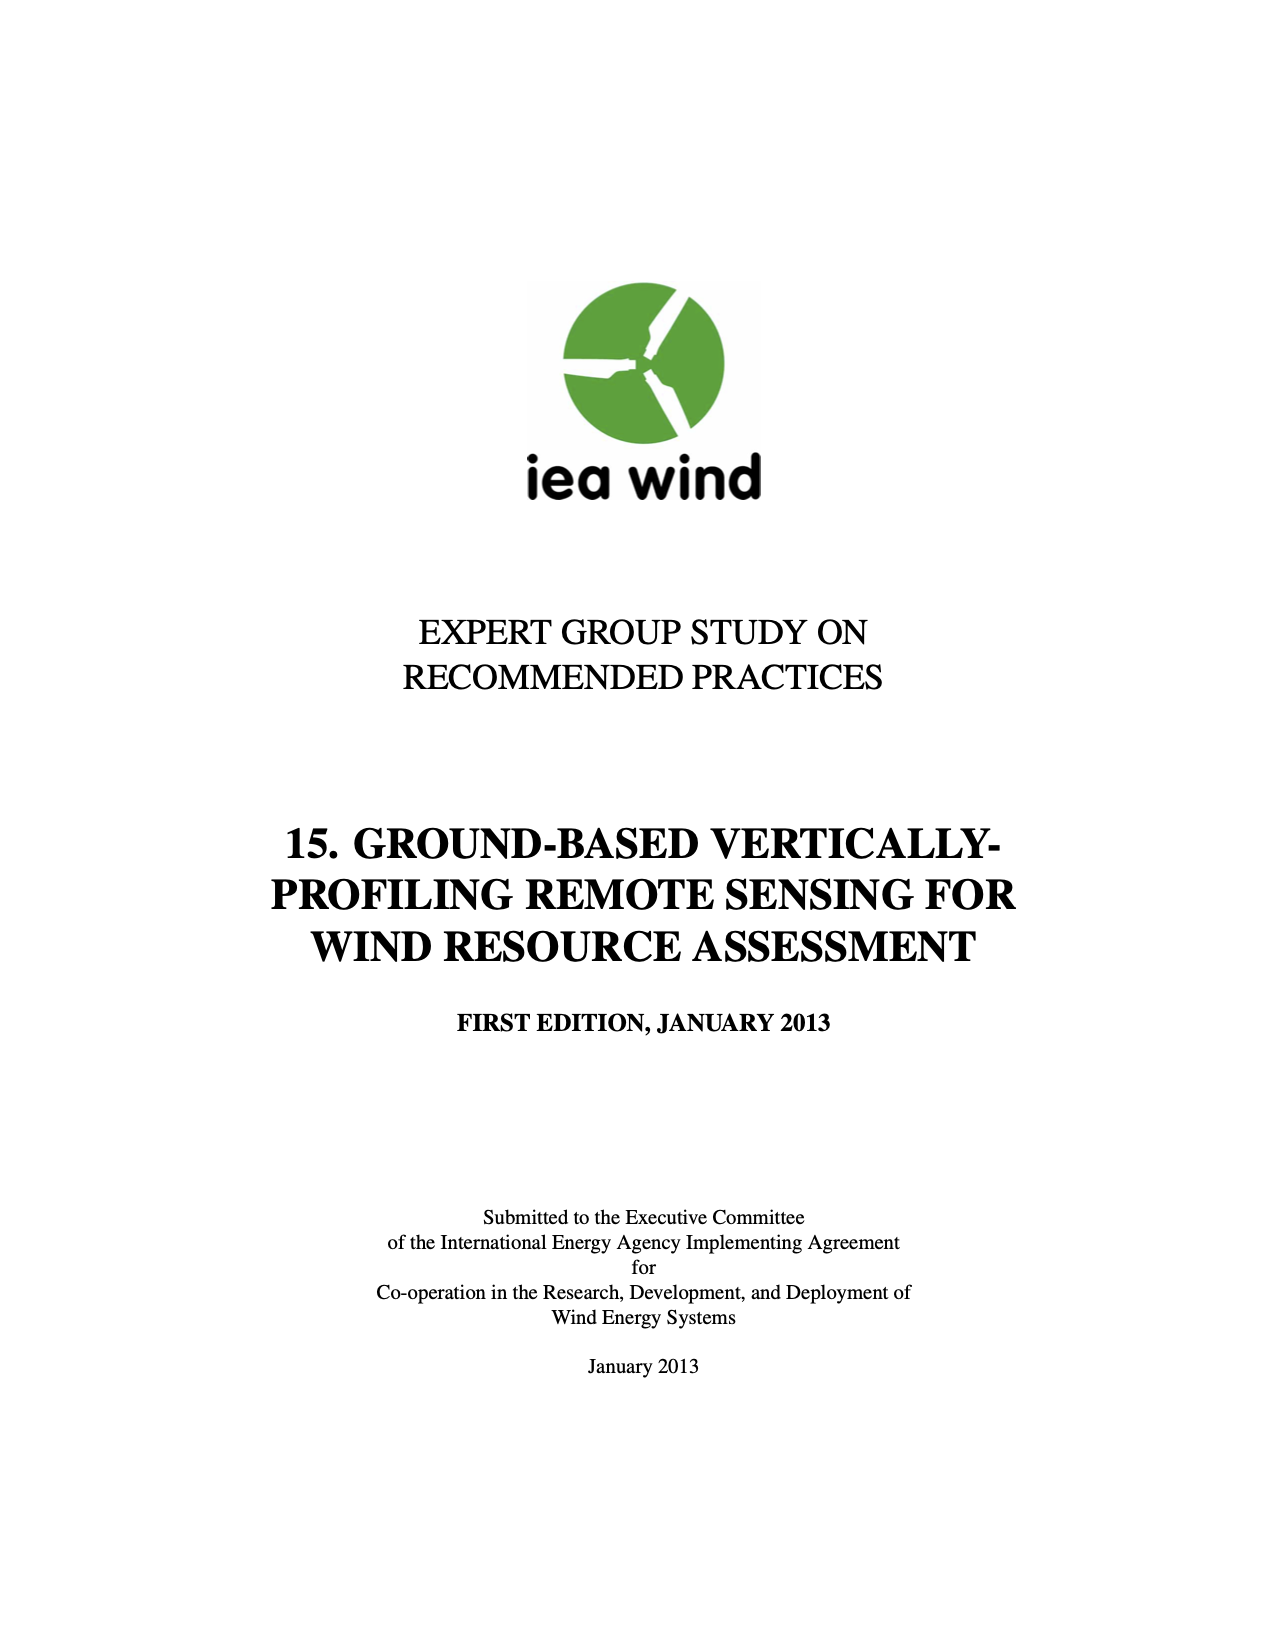
\includegraphics[width=0.9\linewidth, frame]{graphics/RP2013.png}
	% 	\caption{The 2013 Recommended Practices}
	% 	\label{fig:RP15_2013}
	% \end{figure}

In 2017 the International Electrotechnical Committee published a new edition of the IEC 61400-12-1 standard for power performance testing of wind turbines \citep[IEC 61400-12-1 (2017), ][]{IEC_61400_12_1_2017}. The IEC 61400-12-1 standard has traditionally been used as a \emph{de facto} standard for the measurements required for a wind resource assessment. It includes Annex L on the use of remote sensing for wind measurements. As a result, some groups also consider this standard to be applicable to the use case we consider here.

\todo[inline]{Are there other documents we should consider / mention, e.g. TR6?}

%% -----------------------------------
%% What to do in 2020
%% -----------------------------------
\section*{What to do in 2020}
The following sections identify the documents that are applicable at different steps in the lifecycle of a wind lidar deployment:
	
\begin{itemize}
	\item \S \ref{sec:characterizing} Characterising wind lidar
	\item \S \ref{sec:installing} Installing wind lidar
	\item \S \ref{sec:operating} Operating wind lidar
	\item \S \ref{sec:analysis} Lidar data analysis
	\item \S \ref{sec:verification} Verification of wind lidar.
\end{itemize}
	
	%% -----------------------------------
	%% Characterising RSD (RP1)
	%% -----------------------------------

\section{Characterising wind lidar}
\label{sec:characterizing}
It is important that the technology used in the lidar is well characterized for future reference. This is covered in \IEARPndetails{1}{Documentation of RSD characteristics}.

%% -----------------------------------
%% Installing RSD (RP2-16)
%% -----------------------------------

\section{Installing wind lidar}
\label{sec:installing}
\subsection{Training}
Users are encouraged to take specialist training on the wind lidar before deploying the device. This is covered in \IEARPndetails{2}{Training of workers}.

\subsection{Selecting lidar deployment sites}
Careful site selection is important to get high-quality data. There are two important considerations in choosing where the lidar will be placed:

\begin{itemize}
\item \textbf{Avoiding small-scale wind disturbances.} These are phenomena that occur within the wind lidar scanning volume and are not representative of the wind resources at a site. \IEARPn{6 c} recommends avoiding such features.
\item \textbf{Avoiding obstructions.} Wind lidar should have a clear sky view. This is described in \IEARPn{6 d}.
\end{itemize}
  
Some wind lidar devices may be able to ignore small-scale wind disturbances, or still deliver accurate data when the beams are partially obstructed. Therefore users should always follow the manufacturer's guidance on how to site their device.

\todo[inline]{now separating small-scale disturbances from complex terrain}

\subsection{Deploying wind lidar in complex terrain}
\label{sec:complex}
Terrain can influence the winds above it. This may lead to changes in flow within the lidar's measurement volume. This in turn has the effect that the data from a wind lidar may differ from that obtained by a cup anemometer, which is a point measurement and the accepted reference for wind speed measurements. This terrain-induced, measurement-scale flow inhomogeneity is often referred to generally as `complex flow' that occurs in `complex terrain'. It is important to note that the difference between lidar and cup anemometers in complex terrain is influenced by many other factors besides the terrain form. These may include land cover, measurement height, the lidar's own measurement strategy, and weather \cite[amongst others; see e.g.,][]{Clifton_2015_a}.


As noted above, there is no universal, terrain-related boundary between `simple' conditions (where the methods are not beneficial) and `complex' condition. Instead there is a device-specific \textbf{spectrum of complexity} that extends along many axes; terrain form is only one of the axes. At one end of the axes, measurements from a wind lidar are identical to cup anemometers. At the other end, there are observable differences between lidar and point measurements.

\todo[inline]{Not sure about this. Opens the door to too much doubt about lidar performance compared to cups, in general}

Many methods exist that offer to create a transfer function between lidar data and cup anemometer data; we refer to them generically as `transfer methods'. The applicability or suitability of these methods is out of scope for this document.

The fact that each type of device responds differently to winds in complex terrain means that it is not possible to set a guideline for all wind lidar about when to use such methods. Instead, guidelines are needed for each individual type of device.

The major challenge for the user is understanding when to use such transfer methods. Currently the accepted practice is to use a transfer method if advised to do so by the vendor or other experts. However, users may wonder, ``when is it advisable to seek the guidance of an expert?''. In the absence of a directly applicable wind measurement or wind resource assessment standard, we suggest that if conditions are complex according to IEC 61400-12-1 (2017) that it may be appropriate to work with experts to assess the need for such a transfer method. Also, the decision to use such transfer methods -- and the steps required to verify them -- may be driven by the purpose for which the data is being used. Lidar users should always work with their stakeholders to understand their requirements.

An IEA Wind Task 32 working group on the use of wind lidar in complex terrain is carrying out a group study on several different transfer methods. Results are expected in 2021 and the experience gained by this group may lead to the publication of guidelines for this use case.

\todo[inline]{Think this is a bit better than previous version?}
	
\subsection{Transport}
Suggestions for how to prepare and transport lidar are given in \IEARPndetails{4}{Reusable protective packaging for RSD transport} and \IEARPndetails{5}{Installation of shock detectors on the RSD}.
	
\subsection{Site preparation}
Recommendations for site preparation to help ensure a successful deployment are given in \IEARPn{6 a and b}.
	
\subsection{Lidar orientation}
It is important to document the lidar's compass orientation. Recommended practices are given in \IEARPndetails{7}{Device alignment}.
	
\subsection{Tilt and roll}
It is important to monitor the lidar's tilt and roll with respect to  vertical. This may be required for data analysis or to monitor the lidar's stability. Recommended practices are given in \IEARPndetails{8}{Device leveling} and \IEARPndetails{9}{Tilt sensors on the RSD}.
	
\subsection{Time synchronization}
Comparing data from multiple sources (for example, a wind lidar and a traditional tower) requires that the different data be sychronized. Appropriate recommended practices are given in \IEARPndetails{10}{Time sychronization}.
	
\subsection{Power supply}
Many wind lidar devices will be deployed `off the grid'. Recommendations on how to choose a power supply option for such situations are given in \IEARPndetails{11}{Design of remote power systems}. Remote power systems that have any kind of on-site fuel require special care and preparation. Recommended practices are given in \IEARPndetails{12}{Fuelled remote power systems}.
	
\subsection{Protection from interference}
Like any unattended equipment, care should be taken to protect a ground-based lidar from interference. This is covered in \IEARPndetails{13}{Protection from interference}.
	
\subsection{Safety signs and interlocks}
The need for safe operation and signage is covered in \IEARPndetails{14}{safety signs, interlocks and operation}.
	
\subsection{Function check}
It is important to check that the lidar is working properly before being left unattended. A checklist was suggested in \IEARPndetails{15}{Function checklist}. These checks are still useful, but now might be implemented as part of automated tests by the lidar.

\subsection{Stakeholder-driven documentation}
An installation report can add value to the final data set that is used in the wind resource assessment by reducing uncertainty.

The project manager should check that the information in the installation report satisfies all stakeholders and considers future needs. \IEARPndetails{16}{Installation report} describes a possible installation report. Some data users may require additional information about the lidar installation.

\todo[inline]{Changed this title from `installation report' to recognize that some users are quite sophisticated in the information they gather, and some stakeholders need more than that which was listed in \IEARP.}

%% -----------------------------------
%% Operating wind lidar
%% -----------------------------------

\section{Operating wind lidar}
\label{sec:operating}
\subsection{Communications}
\IEARP\ gives recommendations for how to provide remote access to a wind lidar (\IEARPndetails{17}{Remote access to the RSD}).
	
%\subsection{Quantifying sensitivity to ambient conditions}


%If they need such information for their specific use case, lidar users can request a sensitivity analysis that documents the performance of the lidar according to IEC 61400-12-1 (2017) Annex L from the lidar vendor or through a third party. Users should then collect relevant weather data at the deployment site.

\subsection{Deployments in cold climates}
Wind lidar can be deployed in cold climates. In icing conditions they may be easier to keep in operation than wind measurement towers, or could be used together to increase data availability. Like any equipment deployed in cold climates, wind lidar need a reliable power supply, as described in  \IEARPndetails{11}{Design of remote power systems}.

There is an ongoing IEA Wind Task 32 and Task 19 joint effort to share and document experience in using wind lidar in cold climates. Results are expected in 2021 and may lead to the publication of guidelines for this use case.

\todo[inline]{this subsection on cold climates is new}
	
\subsection{Servicing and maintenance}
Like all wind measurement devices, wind lidar may require maintenance from time to time. Recommendations about how wind lidar users and suppliers can work together to ensure reliability and repeatability are provided in \IEARPndetails{23}{Recommended service intervals}.

\subsection{Operation and maintenance log}
Users should keep a log of all use and maintenance of the wind lidar. This is described in \IEARPndetails{24}{Operation and maintenance log}.

%% -----------------------------------
%% Remote sensing data analysis (RP 25-29)
%% -----------------------------------
\section{Remote sensing data analysis}
\label{sec:analysis}

\subsection{Wind speed and vector}
It can be helpful to save data wind lidar data at different steps in the internal data processing. Recommendations for what data to store are given in \IEARPndetails{25}{Line-of-sight wind velocity}, \IEARPndetails{26}{Instantaneous wind vector}, and \IEARPndetails{27}{Time-averaged wind vector}.

\subsection{Turbulence intensity}
Turbulence intensity data are not always required from wind lidar data during wind resource measurements, as these are often obtained from models or other sources.

Because the wind lidar measures wind in a volume, there may be differences between the turbulence intensity measured by a wind lidar compared to a cup anemometer \citep[see e.g.,][]{clifton_2018_a}. As with complex flows (\S \ref{sec:complex}), deriving turbulence intensity from wind lidar is therefore a device-specific challenge.

There have been efforts to create transfer functions for turbulence intensity, but their applicability and suitability is out of the scope of this document. Lidar users may therefore wish to engage with vendors or consultants for guidance.

There are ongoing industry initiatives to explore the use of turbulence data from wind lidar:
\begin{itemize}
  \item The Consortium for the Advancement for Remote Sensing (CFARS, \href{http://www.cfars.org}{www.cfars.org}) is testing several methods of processing wind lidar data to estimate turbulence intensity. Results are expected in mid 2020.
  \item DNV-GL have initiated a joint industry project (JIP; see \href{https://www.dnvgl.com/news/dnv-gl-launches-new-joint-industry-project-to-cut-wind-energy-costs-through-lidar-measurements-154393}{www.dnvgl.com}) to support acceptance and adoption of wind lidar for wind turbulence measurements. Initiated in 2019, the JIP is expected to generate results in 2020 and beyond.
\end{itemize}

\todo[inline]{can we say anything about the validation of such methods? Is it clear (or not) if IEC 61400-12-1 (2017) applies here?}

\subsection{Extreme gusts}
As with turbulence intensity data, extreme gusts measured by wind lidar can also differ from cup anemometers. These differences are also device-specific and as a result, users should engage with vendors and consultants.

\todo[inline]{Feel like we're missing other things in this section, e.g. quality metrics}

%% -----------------------------------
%% Verification of remote sensing devices (RP 30 - 41)
%% -----------------------------------
	%
\section{Verification of remote sensing devices}
\label{sec:verification}
\todo[inline]{Verification or validation? Shouldn't it be validation?  Let's align with IEC..}

All validation activities should be driven by the use case. This was discussed in \IEARP\ Section 1.7 ``A note on `bankability'''.

Users who are interested in exploring the performance of a lidar device could use the approaches set out in \IEARPn{30 -- 40}. However, the methods described in \IEARP\ do not provide the uncertainty information necessary for a wind resource assessment in 2020.

Currently, a wind lidar being used as part of the financing package for a wind energy facility usually undergoes an uncertainty classification according to the IEC 61400-12-1 (2017) standard \cite{IEC_61400_12_1_2017}.

It is expected that the IEC will publish a new wind measurement standard (IEC 61400-50-3) in 2020 or 2021.

\todo[inline]{Trying to say that there are different ways to do a validation test, depending on user needs.}

\section*{Summary}
Many of the 2013 IEA Wind Recommended Practice 15 on Ground-Based Vertically-Profiling Remote Sensing For Wind Resource Assessment are still relevant in 2020, particularly in relation to general good practice when deploying, operating, and maintaining wind lidar.
	
Since 2013 the wind energy community has gathered a huge amount of experience in using wind lidar data. Some of this experience has been captured in the IEC 61400-12-1 Standard for power performance measurements \cite{IEC_61400_12_1_2017}. Upcoming new IEC standards for resource assessment, instrumentation and measurements -- to be published in the 2020's -- may in turn deprecate the 2017 edition of the IEC 61400-12-1 standard for the use case covered in this review.

We anticipate revising this document again during the period 2021-2023 to reflect new developments. Readers are encouraged to check \href{\conceptDOI}{\conceptDOI} for revisions.

%% -----------------------------------
%% Feedback
%% -----------------------------------

\section*{Your feedback and comments}
We welcome constructive feedback about this review and other IEA Wind Task 32 activities:

\begin{itemize}
  \item Feedback \textbf{about the 2013 Recommended Practices} document should be made via \href{https://github.com/IEA-Wind-Task-32/RP15-Ground-Based-Remote-Sensing-for-Wind-Resource-Assessment/issues}{our GitHub repository}.
  \item Feedback \textbf{about this review} should be directed to \href{https://github.com/IEA-Wind-Task-32/RP15-status-update}{the review's GitHub repository} or to the \href{mailto:ieawind.task32@ifb.uni-stuttgart.de}{Task 32 Operating agents}.
\end{itemize}
	
    %% -----------------------------------
    %% References
    %% -----------------------------------
    %\subsection*{References}
    % bibliography
    \label{sec:References}
    \addcontentsline{toc}{section}{References}
    {\small
    \printbibliography
    }
    \vspace*{\fill}


    %% -----------------------------------
    %% Outlined block of smaller text
    %% -----------------------------------
\begin{tcolorbox}[width=1.0\columnwidth,
	boxsep=0pt,
	left=3pt,
	right=3pt,
	top=3pt,
	arc=0pt,
	boxrule=0.5pt,
	toprule=0.5pt,
	colback=white,
	coltext=TextGrey
	]
{%
%% -----------------------------------
%% IEA WIND AND TASK 32
%% -----------------------------------
\noindent%
\footnotesize%
\begin{center}%
\vspace{-2mm}
\begin{tabular}{m{0.3\columnwidth}m{0.6\columnwidth}}
\multicolumn{2}{m{\dimexpr0.9\columnwidth+2\tabcolsep\relax}}{This document was self published by IEA Wind Task 32.}\\
% IEA Wind * DO NOT EDIT THIS TEXT *

\includegraphics[height=2cm]{graphics/IEAWind_logo.jpg}
&
The International Energy Agency is an autonomous organisation which works to ensure reliable, affordable and clean energy for its 30 member countries and beyond. \href{https://community.ieawind.org}{The IEA Wind Technology Collaboration Programme} supports the work of 38 independent, international groups of experts that enable governments and industries from around the world to lead programmes and projects on a wide range of energy technologies and related issues.
\\
% Task 32 * DO NOT EDIT THIS TEXT *
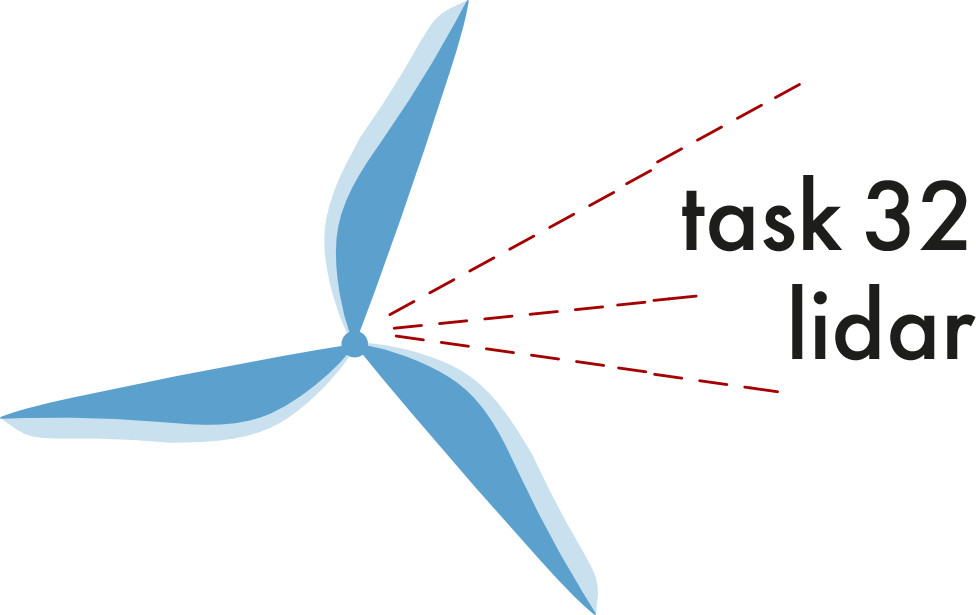
\includegraphics[height=1.5cm]{graphics/Task32_logo.jpg} &
\href{https://community.ieawind.org/task32/home}{IEA Wind Task 32} exists to identify and mitigate the barriers to the deployment of wind lidar for wind energy applications.
\\
%% -----------------------------------
%% More information
%% -----------------------------------
\multicolumn{2}{m{\dimexpr0.9\columnwidth+2\tabcolsep\relax}}{
% N.B. do not add line breaks between the next items
%% -----------------------------------
%% Authors
%% -----------------------------------
\textbf{Author team:} %
Andrew Clifton (Task 32 Operating Agent, University of Stuttgart, Germany), %
Alexander Stoekl (Energiewerkstatt), %
Nicolas Jolin (Nergica),
Paul Mazoyer (Vaisala)
%% -----------------------------------
%% Reviewers
%% -----------------------------------
\textbf{Reviewers:} %
aaa (org x), %
bbb (org y).
%% -----------------------------------
%% Images
%% -----------------------------------
\textbf{Image credits:}
Banner, left to right: \href{https://unsplash.com/@alexkixa}{Alexandre Debiève on Unsplash}, \href{http://ifb.uni-stuttgart.de}{SWE U. Stuttgart}, \href{https://unsplash.com/@markusspiske}{Markus Spiske on Unsplash}.
} % end of more information
\end{tabular}
\end{center}
} % end of footnotesize
\end{tcolorbox} % end of tcolorbox
%% -----------------------------------
%% End of highlighted block
%% -----------------------------------
\vspace*{\fill}

\end{document}
